\documentclass[12pt,a4paper]{article}
\usepackage{geometry}
\usepackage{slashbox}
\geometry{
	a4paper,
	total={170mm,257mm},
	left=20mm,
	right=20mm,
	top=20mm,
	bottom=20mm
}
\usepackage{graphicx}
\usepackage{pdfpages}
\usepackage{placeins}
\usepackage{float}

\usepackage{polski}
\usepackage[utf8]{inputenc}

\begin{document}
	
	\begin{titlepage}
		\newgeometry{top=5.5cm, bottom=3cm}
		
		\centering
		{\huge\bfseries Logika układów cyfrowych lab.\par}
		
		\vspace{0.5cm}
		Prowadzący: Mgr inż. Antoni Sterna (E02-38m, wtorek 17:05) \\
	
		\vspace{1.1cm}
		{\Large sprawozdanie 3 - 2017.10.26\par}
		\vfill
		
		{\large\bfseries Jakub Dorda 235013\par}
		{\large\bfseries Marcin Kotas 235098\par}
		
		\vspace{1cm}
		\today \\ \LaTeX
		
		\restoregeometry
	\end{titlepage}

	
	\section{Wprowadzenie/cel ćwiczeń}
	
	Zapoznanie z podstawami układów sekwencyjnych - rodzajami przerzutników oraz zasadami ich syntezy.
	W pierwszej części ćwiczeń należało zbudować układ sekwencyjny zaprojektowany przez prowadzącego. Po poprawnym wykonaniu
	ćwiczenia, należało przerobić i zrealizować ten sam układ na przerzutnikach typu D. W tym celu należało ponownie wykonać syntezę
	układu oraz minimalizacje.
		
	\section{Układ sekwencyjny (0-5-1-3-2-0) na przerzutnikach JK}
		
		\subsection{Tabela prawdy i tablice Karnaugh:}
			
			\begin{table}[!ht]
			
				\caption{Tabela Prawdy}
				\vspace{0.2cm}
				\centering
				\begin{tabular}{ccc|ccc|cc|cc|cc}
					\multicolumn{3}{c|}{$t$}&\multicolumn{3}{c|}{$t+1$}&$J_2$&$K_2$&$J_1$&$K_1$&$J_0$&$K_0$\\\hline
					0&0&0 &1&0&1 &1&- &0&- &1&-\\
					0&0&1 &0&1&1 &0&- &1&- &-&0\\
					0&1&0 &0&0&0 &0&- &-&1 &0&-\\
					0&1&1 &0&1&0 &0&- &-&0 &-&1\\\hline
					1&0&0 &-&-&- &-&- &-&- &-&-\\
					1&0&1 &0&0&1 &0&1 &0&- &-&0\\
					1&1&0 &-&-&- &-&- &-&- &-&-\\
					1&1&1 &-&-&- &-&- &-&- &-&-\\
				\end{tabular}
				\vspace{1cm}
				
				\begin{minipage}{.5\textwidth}
					\caption{Tablica Karnaugh dla $J_2$}
					\vspace{0.2cm}
					\centering
					\begin{tabular}{c|c|c|c|c}
						\backslashbox{$Q_2$}{$Q_1Q_0$}&00&01&11&10\\\hline
						0&	1&0&0&0\\\hline
						1&	-&-&-&-\\
					\end{tabular}
					
					\vspace{0.4cm}
					
					\caption{Tablica Karnaugh dla $J_1$}
					\vspace{0.2cm}
					\centering
					\begin{tabular}{c|c|c|c|c}
						\backslashbox{$Q_2$}{$Q_1Q_0$}&00&01&11&10\\\hline
						0&	0&1&-&-\\\hline
						1&	-&0&-&-\\
					\end{tabular}
				\end{minipage}%
				\begin{minipage}{.5\textwidth}
				 	\caption{Tablica Karnaugh dla $K_2$}
				 	\vspace{0.2cm}
				 	\centering
				 	\begin{tabular}{c|c|c|c|c}
				 		\backslashbox{$Q_2$}{$Q_1Q_0$}&00&01&11&10\\\hline
				 		0&	-&-&-&-\\\hline
				 		1&	-&1&-&-\\
				 	\end{tabular} 
				 	
			 		\vspace{0.4cm}
			 		
			 		\caption{Tablica Karnaugh dla $K_1$}
			 		\vspace{0.2cm}
			 		\centering
			 		\begin{tabular}{c|c|c|c|c}
			 			\backslashbox{$Q_2$}{$Q_1Q_0$}&00&01&11&10\\\hline
			 			0&	-&-&0&1\\\hline
			 			1&	-&-&-&-\\
			 		\end{tabular} 
				\end{minipage}
				 
			\end{table}
			
			\FloatBarrier
			
			\begin{table}[!ht]
				
				\begin{minipage}{.5\textwidth}
					
					\caption{Tablica Karnaugh dla $J_0$}
					\vspace{0.2cm}
					\centering
					\begin{tabular}{c|c|c|c|c}
						\backslashbox{$Q_2$}{$Q_1Q_0$}&00&01&11&10\\\hline
						0&	1&-&-&0\\\hline
						1&	-&-&-&-\\
					\end{tabular}
				\end{minipage}%
				\begin{minipage}{.5\textwidth}
					
					\caption{Tablica Karnaugh dla $K_0$}
					\vspace{0.2cm}
					\centering
					\begin{tabular}{c|c|c|c|c}
						\backslashbox{$Q_2$}{$Q_1Q_0$}&00&01&11&10\\\hline
						0&	-&0&1&-\\\hline
						1&	-&0&-&-\\
					\end{tabular} 
				\end{minipage}
					
			\end{table}
				
		\subsection{Minimalizacje:}
		
			\begin{minipage}{.5\textwidth}
				
				\begin{displaymath}
					J_2 = \bar{Q_1}\bar{Q_0} = \overline{Q_1 + Q_0}
				\end{displaymath}
				\begin{displaymath}
					J_1 = \bar{Q_2}Q_0 = \overline{Q_2 + \overline{Q_0}}
				\end{displaymath}
				\begin{displaymath}
					J_0 = \bar{Q_1}
				\end{displaymath}
				
			\end{minipage}%
			\begin{minipage}{.5\textwidth}
				
				\begin{displaymath}
					K_2 = 1
				\end{displaymath}
				\begin{displaymath}
					K_1 = \bar{Q_0}
				\end{displaymath}
				\begin{displaymath}
					K_0 = Q_1
				\end{displaymath}
				
			\end{minipage}
			
		\subsection{Użyte wzory:}
		
			\begin{equation}
			\overline{a+b}=\bar{a}\cdot\bar{b}
			\end{equation}
	
		\subsection{Schemat układu:}
		
			\vspace{1.5cm}
			\begin{center}
				\makebox[\textwidth]{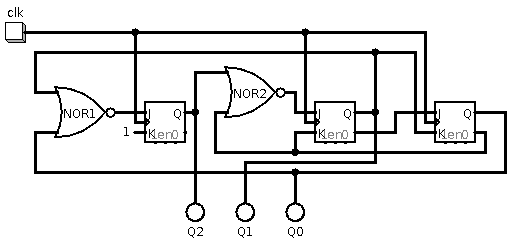
\includegraphics[width=\paperwidth - 40mm]{schem/circuit.png}}
				Schemat 1. Układ sekwencyjny (0-5-1-3-2-0) na przerzutnikach JK
			\end{center}
	
	\section{Układ sekwencyjny (0-5-1-3-2-0) na przerzutnikach D}
		
		\subsection{Tabela prawdy i tablice Karnaugh:}
			
			\begin{table}[H]
				\caption{Tabela Prawdy}
				\vspace{0.2cm}
				\centering
				\begin{tabular}{ccc|ccc|ccc}
					\multicolumn{3}{c|}{$t$}&\multicolumn{3}{c|}{$t+1$}&$D_2$&$D_1$&$D_0$\\\hline
					0&0&0 &1&0&1 &1&0&1\\
					0&0&1 &0&1&1 &0&1&1\\
					0&1&0 &0&0&0 &0&0&0\\
					0&1&1 &0&1&0 &0&1&0\\\hline
					1&0&0 &-&-&- &-&-&-\\
					1&0&1 &0&0&1 &0&0&1\\
					1&1&0 &-&-&- &-&-&-\\
					1&1&1 &-&-&- &-&-&-\\
				\end{tabular}
				\vspace{1cm}
				
				\begin{minipage}{.5\textwidth}
					\caption{Tablica Karnaugh dla $D_2$}
					\vspace{0.2cm}
					\centering
					\begin{tabular}{c|c|c|c|c}
						\backslashbox{$Q_2$}{$Q_1Q_0$}&00&01&11&10\\\hline
						0&	1&0&0&-\\\hline
						1&	-&0&-&0\\
					\end{tabular}
					
					\vspace{0.4cm}
					
					\caption{Tablica Karnaugh dla $D_1$}
					\vspace{0.2cm}
					\centering
					\begin{tabular}{c|c|c|c|c}
						\backslashbox{$Q_2$}{$Q_1Q_0$}&00&01&11&10\\\hline
						0&	0&1&1&0\\\hline
						1&	-&0&-&-\\
					\end{tabular}
				\end{minipage}%
				\begin{minipage}{.5\textwidth}
					\caption{Tablica Karnaugh dla $D_0$}
					\vspace{0.2cm}
					\centering
					\begin{tabular}{c|c|c|c|c}
						\backslashbox{$Q_2$}{$Q_1Q_0$}&00&01&11&10\\\hline
						0&	1&1&0&0\\\hline
						1&	-&1&-&-\\
					\end{tabular} 
					
				\end{minipage}
			\end{table}
	
		\subsection{Minimalizacje:}
			
			\begin{displaymath}
			D_2 = \bar{Q_1}\bar{Q_0} = \overline{Q_1 + Q_0}
			\end{displaymath}
			\begin{displaymath}
			D_1 = \bar{Q_2}Q_0 = \overline{Q_2 + \overline{Q_0}}
			\end{displaymath}
			\begin{displaymath}
			D_0 = \bar{Q_1}
			\end{displaymath}
			
		\subsection{Użyte wzory:}
		
			\begin{equation}
			\overline{a+b}=\bar{a}\cdot\bar{b}
			\end{equation}
			
		\subsection{Schemat układu:}
		
			\vspace{0.5cm}
			\begin{center}
				\makebox[\textwidth]{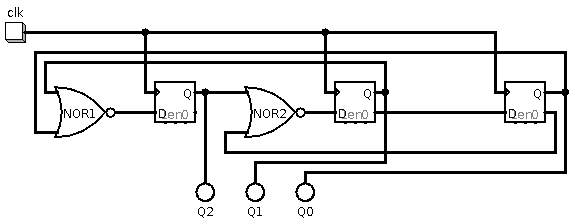
\includegraphics[width=\paperwidth - 40mm]{schem/circuit2.png}}
				Schemat 2. Układ sekwencyjny (0-5-1-3-2-0) na przerzutnikach D
			\end{center}

	\section{Wnioski/podsumowanie}
	
		W celu sprawdzenia poprawności działania należało przeprowadzić testy dla wszystkich możliwych kombinacji wyjść, czyli
		przejść przez cały cykl działania układu. Wykonanie pierwszego ćwiczenia sprawiło trudności z powodu spięcia wywołanego 
		przez błąd konstrukcyjny zestawu Unilog (zwarcie między płytką a obudową zestawu). Przez problemy techniczne nie udało się
		wykonać drugiego układu w czasie trwania laboratorium. Poprawiona synteza i minimalizacja oraz układ dla drugiej części
		ćwiczeń zostały zawarte w sprawozdaniu 

\end{document}